\section{Projekt Stanowisk Komputerowych - Specyfikacja}

\subsection{Specyfikacja Stacji Roboczych}

    Opis specyfikacji stacji roboczych:\\
    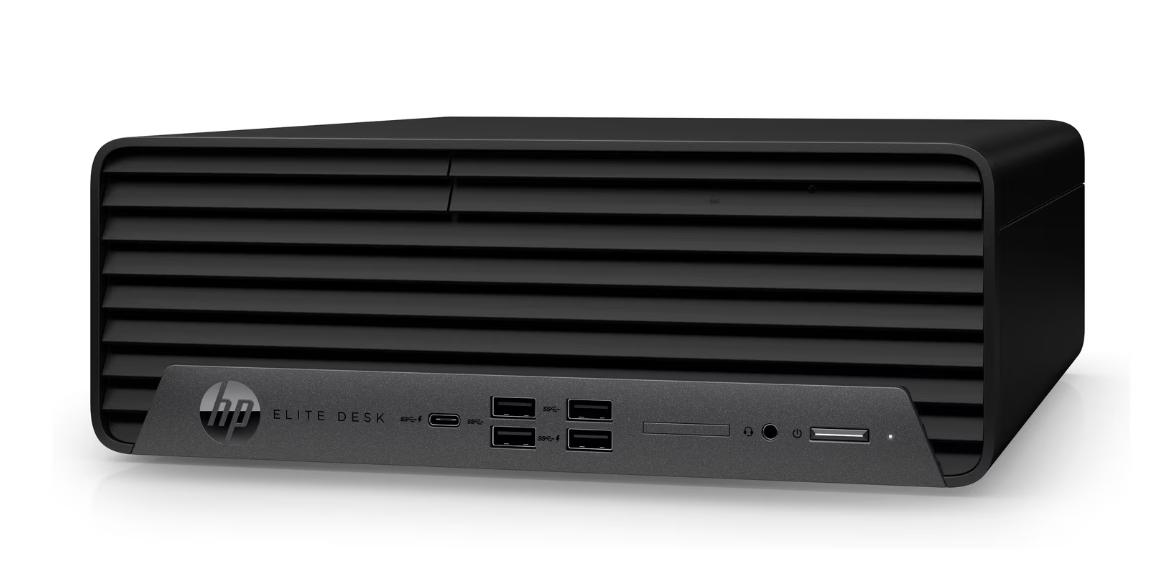
\includegraphics[width=0.5\textwidth]{sprzet/elitedesk}
    \begin{flushleft}
        \begin{table}[h]
            \renewcommand{\arraystretch}{1.5}
            \begin{tabular}{|l|l|}
            \hline
                \textbf{Parametr} & \textbf{Specyfikacja} \\
            \hline
                Model & HP EliteDesk 800 G7 \\
                Procesor & Intel Core i7-12700 \\
                Pamięć RAM & 32 GB DDR4 \\
                Dysk twardy & 1 TB SSD \\
                Karta graficzna & NVIDIA GeForce GTX 3070 \\
                System operacyjny & Windows 11 Pro \\
            \hline
            \end{tabular}
        \end{table}  
    \end{flushleft}

\subsection{Stacje Administracyjne}

    Opis specyfikacji stacji Administracyjnej:\\
    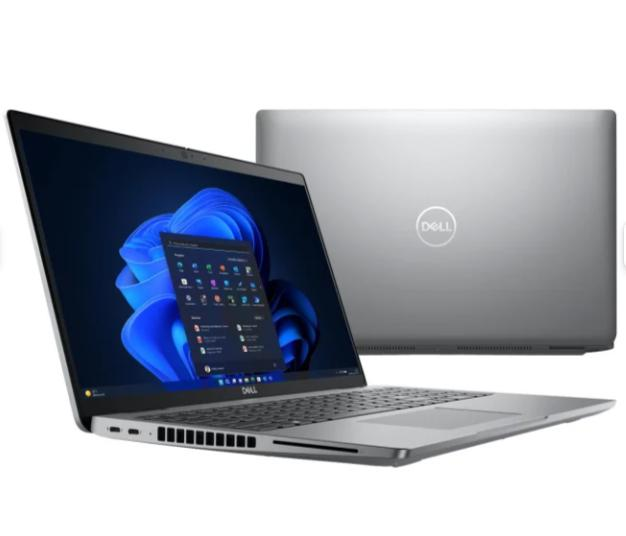
\includegraphics[width=0.3\textwidth]{sprzet/laptop}


    \begin{flushleft}
        \begin{table}[h]
            \renewcommand{\arraystretch}{1.5}
            \begin{tabular}{|l|l|}
            \hline
                \textbf{Parametr} & \textbf{Specyfikacja} \\
            \hline
                Model & Dell Latitude 5540\\
                Procesor & i5-1335U \\
                Pamięć RAM & 16 GB DDR4 \\
                Dysk twardy & 512 GB SSD \\
                Karta graficzna & Intel Iris Xe Graphics \\
                System operacyjny & Windows 11 Pro + Ubuntu 22.04 LTS \\
            \hline
            \end{tabular}
        \end{table}  
    \end{flushleft}
\pagebreak

\subsection{Serwer Plików}

    Opis specyfikacji:\\
    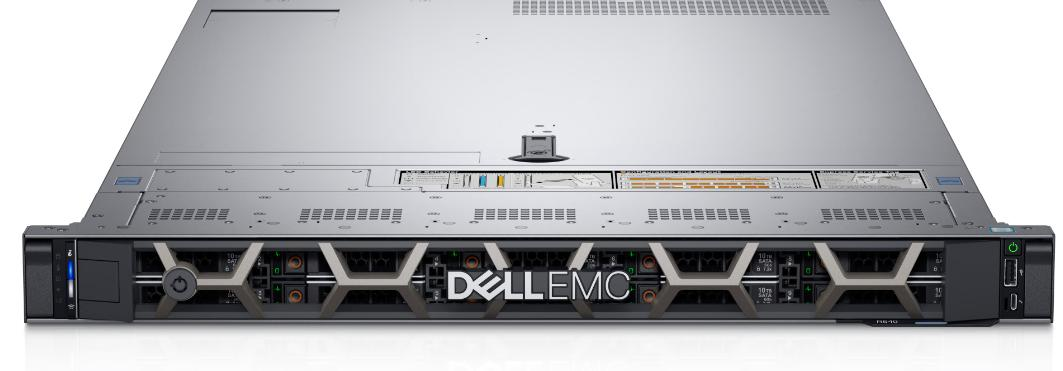
\includegraphics[width=0.3\textwidth]{sprzet/dell-serwer}

    \begin{flushleft}
        \begin{table}[h]
            \renewcommand{\arraystretch}{1.5}
            \begin{tabular}{|l|l|}
            \hline
                \textbf{Parametr} & \textbf{Specyfikacja} \\
            \hline
                Model & Dell PowerEdge R640 \\
                Procesor & 2x Intel Gold 6140 2.3Ghz1 8-Core \\
                Pamięć RAM & 256GB RAM DDR4 2666Mhz \\
                Dysk twardy & 2x 960GB SATA SSD + 6x 1.2TB SAS 10k \\
                System operacyjny & Windows Server 2022 \\
            \hline
            \end{tabular}
        \end{table}  
    \end{flushleft}

\subsection{Monitor}

    Opis specyfikacji:\\
    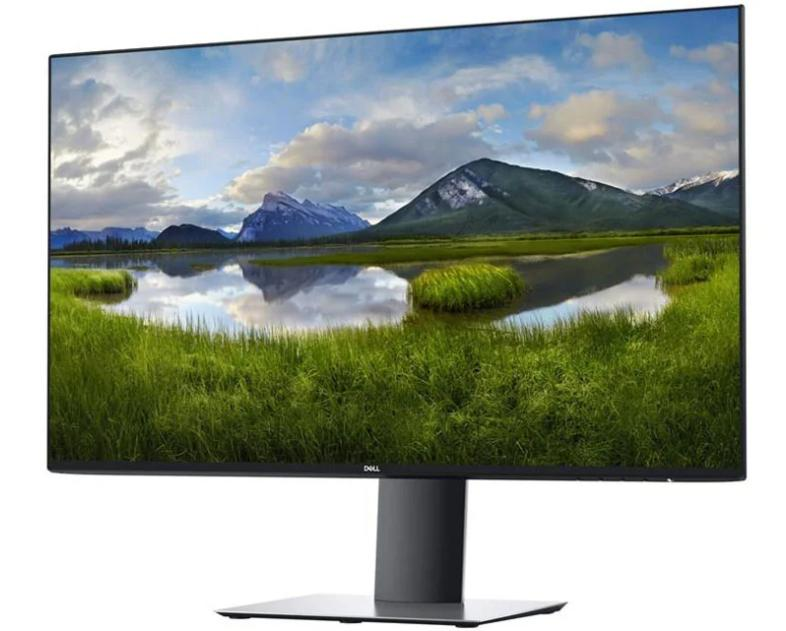
\includegraphics[width=0.3\textwidth]{sprzet/monitor}

    \begin{flushleft}
        \begin{table}[h]
            \renewcommand{\arraystretch}{1.5}
            \begin{tabular}{|l|l|}
            \hline
                \textbf{Parametr} & \textbf{Specyfikacja} \\
            \hline
                Model & Monitor Dell UltraSharp 27 — U2722D            \\
                Przekątna & 27 cali \\
                Rozdzielczość & QHD 60 Hz \\
                Panel & IPS \\
            \hline
            \end{tabular}
        \end{table}  
    \end{flushleft}

\subsection{Drukarka Sieciowa i Skaner}

    Specyfikacje drukarki sieciowej:\\
    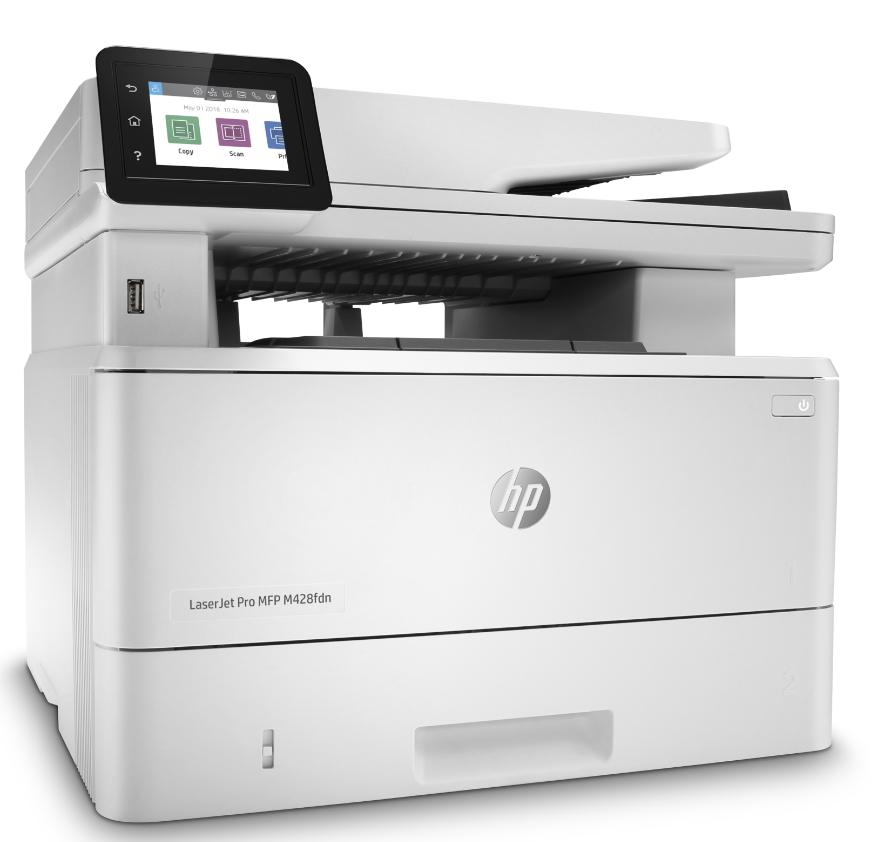
\includegraphics[width=0.3\textwidth]{sprzet/drukarka}

    \begin{flushleft}
        \begin{table}[h]
            \renewcommand{\arraystretch}{1.5}
            \begin{tabular}{|l|l|}
            \hline
            \textbf{Urządzenie} & \textbf{Specyfikacja} \\
            \hline
                Drukarka Sieciowa & HP LaserJet Pro MFP M428fdn \\
                Rodzaj drukarki & Monochromatyczna laserowa \\
                Funkcje & Druk, skanowanie, kopiowanie, faks \\
                Prędkość druku & Do 40 str./min \\
            \hline
            \end{tabular}
        \end{table}
    
    \end{flushleft}

\pagebreak

\subsection{Akcesoria oraz inne peryferia lub urządzenia}

    \begin{flushleft}
        \begin{table}[h]
            \renewcommand{\arraystretch}{1.5}
            \begin{tabular}{|l|l|}
            \hline
            \textbf{Urządzenie} & \textbf{Model} \\
            \hline
                Klawiatura oraz myszka bezprzewodowa & Dell Pro Keyboard and Mouse KM5221W \\
                Projektor & BenQ MX560 DLP \\
                Kabel sygnałowy & Silver Monkey Kabel HDMI 2.0 - HDMI 3m\\
                Skaner & Epson Perfection V600 Photo \\


            \hline
            \end{tabular}
        \end{table}

    \end{flushleft}    